\tikzset{XOR/.style={draw,circle,append after command={
		[shorten >=\pgflinewidth, shorten <=\pgflinewidth,]
		(\tikzlastnode.north) edge (\tikzlastnode.south)
		(\tikzlastnode.east) edge (\tikzlastnode.west)
		}
	}
}

\chapter{Sicherheit - Verfahren und Formelsammlung}

Zusammenfassung der Vorlesung "`Sicherheit"' aus dem Sommersemester 2016.\footnote{\url{https://crypto.iti.kit.edu/index.php?id=sic-sose16}}

Der Lehrstuhl stellt bereits ein ausführliches Skript zur Verfügung.\footnote{\url{https://github.com/skript-sicherheit/skript}}. Die hier verwendeten Grafiken sind im Wesentlichen von dort entnommen.

\section{Einleitung}



\section{Symmetrische Verschlüsselung}

\subsection{Stromchiffren}

\subsubsection{One-Time-Pad}
\begin{itemize}
	\item Verschlüsselung einer Nachricht \(M\) mit einem Schlüssel \(K\) der selben Länge: \(C = M \oplus K, |M| = |K|\)
	\item \(K\) muss zufällig gleichverteilt gezogen werden und darf nicht mehrfach verwendet werden
	\item Vorteil: Perfekte Geheimhaltung, da sich aus \(C\) keine Informationen über \(M\) ableiten lassen
	\item \textbf{Nachteile}
	\begin{itemize}
		\item Bei Wiederverwenden des selben Schlüssels angreifbar: \(C_1 \oplus C_2 = M_1 \oplus K \oplus K \oplus M_2 = M_1 \oplus M_2\)
		\item Verdoppelter Übertragungsaufwand (unhandlich)
	\end{itemize}
\end{itemize}


\subsection{Blockchiffren}

\subsubsection{Verschlüsselungsverfahren}
\begin{itemize}
	\item Blockweise Aufteilung und Verschlüsselung: \(ENC: \big\{0,1\big\}^k \times \big\{0,1\big\}^l \rightarrow \big\{0,1\big\}^l\)
	\item \textbf{Designkriterien}
	\begin{itemize}
		\item \textit{Diffusion} bzw. Nichtunterscheidbarkeit von echt zufälligen Funktionen: Kleine Änderungen an der Eingabe müssen im Mittel zu großen Veränderungen bei der Ausgabe führen
		\item \textit{Confusion}: Jedes Zeichen des Chiffrats ist von mehreren Zeichen des Schlüssels abhängig
	\end{itemize}
\end{itemize}

\begin{figure}[h]
	\centering
	\tikzstyle{encrypt}=[draw,fill=black!15,rectangle,minimum size=20pt,inner sep=0pt]
	\tikzstyle{every circle node}= [draw]
	\begin{tikzpicture}
		\begin{scope}[>=latex] %for filled arrow tips
			\newcommand{\n}{3}
			\draw [decorate,decoration={brace,amplitude=10pt},xshift=0,yshift=0pt] (6.5, {(\n -1)*2 + 2.25}) -- (6.5,-3.25) node [black,midway,xshift=28.0, yshift=0.0] {$ENC$};
	
			\node (rectM) at (2, {(\n -1)*2 + 2}) [draw,thick,minimum width=8cm, minimum height=0.5cm] {$M$};
			\node (rect1) at (0, {(\n -1)*2 + 1}) [draw,thick,minimum width=4cm, minimum height=0.5cm] {$L_0$};
			\node (rect2) at (4, {(\n -1)*2 + 1}) [draw,thick,minimum width=4cm, minimum height=0.5cm] {$R_0$};
			\draw[->,semithick] (rectM) -- (2, {(\n -1)*2 + 1.30});
			\foreach \nr in {1, ..., \n}{
				\node (x\nr)[XOR] at (0,{(\n-\nr)*2}) {};
				\node (F\nr)[encrypt] at (2.0, {(\n-\nr)*2}) {$F_\nr$};
				\draw[->,semithick] (F\nr) -- (x\nr);
			}
			\node (rectL3) at (0, -2.0) [draw,thick,minimum width=4cm, minimum height=0.5cm] {$L_3$};
			\node (rectR3) at (4, -2.0) [draw,thick,minimum width=4cm, minimum height=0.5cm] {$R_3$};
			% draw first connection lines
			\draw[->,semithick] (rect1) -- (x1);
			\draw[->, semithick] (rect2) |- (F1);
			% \node (p1)[circle, fill, inner sep=0cm, minimum size=0.12cm] at (4, {(\n-1)*2}) {};
			% \draw[->, semithick] (p1) -- (F1);
	
			% draw connection lines between F-Boxes
			\foreach \nr in {1, ..., 2}{
				\pgfmathsetmacro\cnr{int(\nr + 1)}
				\node (p\nr)[circle, fill, inner sep=0cm, minimum size=0.12cm] at (4, {(\n-\nr)*2}) {};
				\draw[->, semithick] (p\nr) -- (4, {(\n-\nr)*2 - 0.6}) -- (0, {(\n-\nr)*2 - 1.2}) -- (x\cnr);
		
				\draw[->, semithick] (x\nr) -- (0, {(\n-\nr)*2 - 0.6}) -- (4, {(\n-\nr)*2 - 1.2}) |- (F\cnr);
			}
			\draw[->, semithick] (x3) -- (0, {(\n-3)*2 - 0.6}) -- (4, {(\n-3)*2 - 1.2}) -- (rectR3);
	
			\node (p3)[circle, fill, inner sep=0cm, minimum size=0.12cm] at (4, {(\n-3)*2}) {};
			\draw[->, semithick] (p3) -- (4, {(\n-(3))*2 - 0.6}) -- (0, {(\n-(3))*2 - 1.2}) -- (rectL3);
	
			\node (rectC) at (2, -3) [draw,thick,minimum width=8cm, minimum height=0.5cm] {$C$};
			\draw[->,semithick] (2, -2.25) -- (rectC);
	
		\end{scope}
	\end{tikzpicture}
	\caption{3-ründige Feistel-Struktur}
\end{figure}
\FloatBarrier

\subsubsection{Betriebsmodi}

\paragraph{Electronic Codebook Mode (ECB-Modus)}
Alle Nachrichtenblöcke werden unabhängig voneinander, mit dem selben Schlüssel verschlüsselt \(\rightarrow\) identische Klartextblöcke liefern identische Chiffratblöcke.

\begin{figure}[h]
	\centering
	\begin{subfigure}[h]{.45\textwidth}
		\centering
		\tikzstyle{vertex}=[draw,fill=black!15,circle,minimum size=20pt,inner sep=0pt]
		\tikzstyle{encrypt}=[draw,fill=black!15,rectangle,minimum width=1cm, minimum height=0.65cm,inner sep=0pt]
		\begin{tikzpicture}
			\begin{scope}[>=latex]
				\newcommand{\n}{3}
				\foreach \nr in {1, ..., \n}{
					\node (M\nr) at (0,{(\n-\nr)*2}) {$M_\nr$};
					\node (C\nr) at (4,{(\n-\nr)*2}) {$C_\nr$};
					\node (E\nr)[encrypt] at (2,{(\n-\nr)*2}) {ENC};
					\node (K\nr) at (2,{(\n-\nr)*2+1}) {K};
					
					\draw[->,semithick] (M\nr) -- (E\nr);
					\draw[->,semithick] (K\nr) -- (E\nr);
					\draw[->,semithick] (E\nr) -- (C\nr);
				}
			\end{scope}
		\end{tikzpicture}
		\caption{Verschlüsselung im ECB-Modus.}
	\end{subfigure}
	\hfill
	\begin{subfigure}[h]{.45\textwidth}
		\centering
		\tikzstyle{vertex}=[draw,fill=black!15,circle,minimum size=20pt,inner sep=0pt]
		\tikzstyle{encrypt}=[draw,fill=black!15,rectangle,minimum width=1cm, minimum height=0.65cm,inner sep=0pt]
		\begin{tikzpicture}
			\begin{scope}[>=latex]
				\newcommand{\n}{3}
				\foreach \nr in {1, ..., \n}{
					\node (M\nr) at (0,{(\n-\nr)*2}) {$M_\nr$};
					\node (C\nr) at (4,{(\n-\nr)*2}) {$C_\nr$};
					\node (E\nr)[encrypt] at (2,{(\n-\nr)*2}) {DEC};
					\node (K\nr) at (2,{(\n-\nr)*2+1}) {K};
					
					\draw[->,semithick] (M\nr) -- (E\nr);
					\draw[->,semithick] (K\nr) -- (E\nr);
					\draw[->,semithick] (E\nr) -- (C\nr);
				}
			\end{scope} 
		\end{tikzpicture}
		\caption{Entschlüsselung im ECB-Modus.}
	\end{subfigure}
\end{figure}
\FloatBarrier

\paragraph{Cipher Block Chaining Mode (CBC-Modus)}
\begin{itemize}
	\item Jeder Block wird zusätzlich mit dem Ergebnis des davor liegenden Block "`vorverschlüsselt"'
	\item Bitfehler innerhalb eines Blocks wirken sich bei der Entschlüsselung nur auf diesen und den nachfolgenden Block aus (selbstkorrigierend)
	\item Entschlüsselung kann parallelisiert werden (Verschlüsselung nicht)
\end{itemize}

\begin{figure}[h]
	\begin{subfigure}[h]{.45\textwidth}
		\centering
		\tikzstyle{encrypt}=[draw,fill=black!15,rectangle,minimum width=1cm, minimum height=0.65cm,inner sep=0pt]
		\begin{tikzpicture}
			\begin{scope}[>=latex]
				\newcommand{\n}{3}
				\foreach \nr in {1, ..., \n}{
					\node (M\nr)            at (0,{(\n-\nr)*2}) {$M_\nr$};
					\node (x\nr)[XOR]       at (2,{(\n-\nr)*2}) {};
					\node (E\nr)[encrypt]   at (4,{(\n-\nr)*2}) {ENC};
					\node (C\nr)            at (6,{(\n-\nr)*2}) {C};
					
					\node (K\nr)            at (4,{(\n-\nr)*2+1}) {K};
					
					\draw[->,semithick] (M\nr) -- (x\nr);
					\draw[->,semithick] (x\nr) -- (E\nr);
					\draw[->,semithick] (E\nr) -- (C\nr);
					
					\draw[->,semithick] (K\nr) -- (E\nr);
				}
				
				\foreach \nr in {2, ..., \n}{
					\pgfmathtruncatemacro{\tmp}{\nr-1}
					\node (p\tmp)[circle, fill, inner sep=0cm, minimum size=0.12cm] at (5.0, {(\n-\tmp)*2}) {};
					\draw[->,semithick] (p\tmp) -- (5.0, {(\n-\tmp)*2-0.5}) -- (2, {(\n-\nr)*2+1.5}) -- (x\nr);
				}
				
				\node (IV) at (2,{\n*2-1}) {$IV$};
				\draw[->,semithick] (IV) -- (x1);
			\end{scope}
		\end{tikzpicture}
		\caption{Verschlüsselung im CBC-Modus.}
	\end{subfigure}
	\hfill
	\begin{subfigure}[h]{.45\textwidth}
		\centering
		\tikzstyle{encrypt}=[draw,fill=black!15,rectangle,minimum width=1cm, minimum height=0.65cm,inner sep=0pt]
		\begin{tikzpicture}
			\begin{scope}[>=latex]
				\newcommand{\n}{3}
				\foreach \nr in {1, ..., \n}{
					\node (C\nr)            at (0,{(\n-\nr)*2}) {$C_\nr$};
					\node (D\nr)[encrypt]   at (2,{(\n-\nr)*2}) {DEC};
					\node (x\nr)[XOR]       at (4,{(\n-\nr)*2}) {};
					\node (M\nr)            at (6,{(\n-\nr)*2}) {$M_\nr$};
					
					\node (K\nr)            at (2,{(\n-\nr)*2+1}) {K};
					
					\draw[->,semithick] (C\nr) -- (D\nr);
					\draw[->,semithick] (D\nr) -- (x\nr);
					\draw[->,semithick] (x\nr) -- (M\nr);
					
					\draw[->,semithick] (K\nr) -- (D\nr);
				}
				
				\foreach \nr in {2, ..., \n}{
					\pgfmathtruncatemacro{\tmp}{\nr-1}
					\node (p\tmp)[circle, fill, inner sep=0cm, minimum size=0.12cm] at (1.0, {(\n-\tmp)*2}) {};
					\draw[->,semithick] (p\tmp) -- (1,{(\n-\tmp)*2-0.5}) -- (4,{(\n-\tmp)*2-0.5}) -- (x\nr);
				}
				
				\node (IV) at (4,{\n*2-1}) {$IV$};
				\draw[->,semithick] (IV) -- (x1);
			\end{scope}
		\end{tikzpicture}
		\caption{Entschlüsselung im CBC-Modus.}
	\end{subfigure}
\end{figure}
\FloatBarrier

\paragraph{Counter Mode (CTR-Modus)}
Bietet die Vorteile des CBC-Modus und kann parallelisiert werden.

\begin{figure}[h]
	\centering
	\begin{subfigure}[h]{.45\textwidth}
		\centering
		\tikzstyle{encrypt}=[draw,fill=black!15,rectangle,minimum width=1cm, minimum height=0.65cm,inner sep=0pt]
		\begin{tikzpicture}
			\begin{scope}[>=latex] %for filled arrow tips
				\newcommand{\n}{3}
				\foreach \nr in {1, ..., \n}{
					\node (M\nr) at (0,{(\n-\nr)*3}) {$M_\nr$};
					\node (x\nr)[XOR] at (2,{(\n-\nr)*3}) {};
					\node (E\nr)[encrypt] at (2,{(\n-\nr)*3+1}) {ENC};
					\node (K\nr) at (2,{(\n-\nr)*3+2}) {K};
					\node (C\nr) at (4,{(\n-\nr)*3}) {$C_\nr$};
					\draw[->,semithick] (M\nr) -- (x\nr);
					\draw[->,semithick] (x\nr) -- (C\nr);
					\draw[->,semithick] (K\nr) -- (E\nr);
					\draw[->,semithick] (E\nr) -- (x\nr);
				}
				\foreach \nr in {1, ..., \n}{
					\node (IV\nr) at (0.38,{(\n - \nr)*3+1}) {$IV+\nr$};
					\draw[->,semithick] (IV\nr) -- (E\nr);
				}
			\end{scope}
		\end{tikzpicture}
		\caption{Verschlüsselung im CTR-Modus.}
	\end{subfigure}
	\hfill
	\begin{subfigure}[h]{.45\textwidth}
		\centering
		\tikzstyle{encrypt}=[draw,fill=black!15,rectangle,minimum width=1cm, minimum height=0.65cm,inner sep=0pt]
		\begin{tikzpicture}
			\begin{scope}[>=latex] %for filled arrow tips
				\newcommand{\n}{3}
				\foreach \nr in {1, ..., \n}{
					\node (C\nr) at (0,{(\n-\nr)*3}) {$C_\nr$};
					\node (x\nr)[XOR] at (2,{(\n-\nr)*3}) {};
					\node (E\nr)[encrypt] at (2,{(\n-\nr)*3+1}) {ENC};
					\node (K\nr) at (2,{(\n-\nr)*3+2}) {K};
					\node (M\nr) at (4,{(\n-\nr)*3}) {$M_\nr$};
					\draw[->,semithick] (C\nr) -- (x\nr);
					\draw[->,semithick] (x\nr) -- (M\nr);
					\draw[->,semithick] (K\nr) -- (E\nr);
					\draw[->,semithick] (E\nr) -- (x\nr);
				}
				\foreach \nr in {1, ..., \n}{
					\node (IV\nr) at (0.38,{(\n - \nr)*3+1}) {$IV+\nr$};
					\draw[->,semithick] (IV\nr) -- (E\nr);
				}
			\end{scope}
		\end{tikzpicture}
		\caption{Entschlüsselung im CTR-Modus.}
	\end{subfigure}
\end{figure}
\FloatBarrier

\paragraph{Galois/-Counter Mode (GCM-Modus)}
Berechnet neben dem Chiffrat zusätzlich eine Signatur, um die Integrität sicherzustellen.



\section{Kryptografische Sicherheitsbegriffe}

\subsection{Sicherheitsparameter und effiziente Angreifer}
\begin{itemize}
	\item Sicherheitsniveau \(k\) legt mit der Definition des Schlüsselraums \(1^k\) das Sicherheitsniveau einer Funktion fest
	\item Effizienter Angreifer: Muss in \(\mathcal{O}\big(k^c\big), c \in \mathbb{N}\). Dies schließt so beispielsweise einen Brute-Force-Angriff auf den kompletten Schlüsselraum \(\{0,1\}^k\) mit \(\mathcal{O}\big(2^k\big)\) aus
	\item PPT-Angreifer: Verwendet probabilistische Angriffe ("`probabilistic polynomial time"')
\end{itemize}


\subsection{Semantische Sicherheit}


\subsection{Der IND-CPA-Sicherheitsbegriff}
\begin{itemize}
	\item \textit{Undistinguishability unser chosen-plaintext attacks}: Ein polynomiell bschränkter Angreifer \(\mathcal{A}\) kann nicht Chiffrate nicht von selbst gewählen (und verschlüsselten) Klartexten unterscheiden
	\item Einführung eines Verschlüsselungsorakels (\(\mathcal{A}\) kann zu jedem Zeitpunkt jedes beliebige \(M\) verschlüsseln lassen) und eines Herausforderers \(\mathcal{C}\)
	\item \textbf{Vorgehen}
	\begin{enumerate}
		\item \(\mathcal{A}\) wählt zwei Nachrichten \(M_1\) und \(M_2\) mit \(M_1 \neq M_2\) und \(|M_1| = |M_2|\)
		\item \(\mathcal{C}\) verschlüsselt zufällig \(M_b\) mit \(b \in \{1,2\}\)
		\item \(\mathcal{A}\) gewinnt, wenn er \(b\) mit Hilfe des Orakels korrekt rät
	\end{enumerate}
\end{itemize}



\section{Hashfunktionen}

\subsection{Grundlagen}
Funktionen die von einer großen, potentiell unbeschränkten Menge in eine kleinere Menge abbilden:
\[H_k : \{0,1\}^* \leftarrow \{0,1\}^k\]


\subsection{Sicherheitseigenschaften}
\begin{itemize}
	\item Kollisionsresistenz: Es soll schwierig sein, zwei unterschiedliche Urbilder \(X\) und \(X'\) zu finden, für die \(X \neq X'~\text{und}~H(X) = H(X')\) gilt
	\item Einwegeingeschaft: Zu jedem gegebenen Wert \(H(X)\) soll es schwierig sein, ein passendes \(X\) zu finden
	\item Jede kollisionsresistente Hashfunktion ist eine Einwegfunktion
\end{itemize}


\subsection{Merkle-Damg\r{a}rd-Transformation}
\begin{itemize}
	\item Zusätzlichen zu den beschriebenen Eigenschaften müssen Hashfunktionen in der Praxis bei flexibler Eingabelänge konstant in ihrer Ausgabelänge sein
	\item Zunächst Aufteilung der Eingabe in Blöcke der Länge \(l\) (der hinterste Block wird ggf. gepattet), auf diese anschließend nacheinander die Kompressionsfunktion \(F: \{0,1\}^{l+k} \leftarrow \{0,1\}^k\) angewendet wird
	\item Der Initialisierungsvektor wird für jede Hashfunktion fest gewählt
	\item Die Sicherheit der Transformation \(H_{MD}\) hängt stark von der verwendeten Kompressionsfunktion ab
\end{itemize}

\begin{figure}[h]
	\begin{center}
		\unitlength=1mm
		\linethickness{0.4pt}
		\begin{picture}(110,20)

			\put(5,5){\vector(1,0){15}}
			\put(12,6){\makebox(0,0)[cb]{IV}}

			\put(25,15){\vector(0,-1){7.5}}
			\put(28,10){\makebox(0,0)[cb]{$M_1$}}

			\put(20,2.5){\framebox(10,5){$F$}}

			\put(30,5){\vector(1,0){12}}
			\put(36,6){\makebox(0,0)[cb]{$Z_1$}}

			\put(47,15){\vector(0,-1){7.5}}
			\put(50,10){\makebox(0,0)[cb]{$M_2$}}

			\put(42,2.5){\framebox(10,5){$F$}}

			\put(52,5){\vector(1,0){12}}
			\put(58,6){\makebox(0,0)[cb]{$Z_2$}}

			\put(68,4){\makebox(0,0)[cb]{\ldots}}

			\put(72,5){\vector(1,0){12}}
			\put(78,6){\makebox(0,0)[cb]{$Z_{n-1}$}}

			\put(84,2.5){\framebox(10,5){$F$}}

			\put(89,15){\vector(0,-1){7.5}}
			\put(92,10){\makebox(0,0)[cb]{$M_{n}$}}

			\put(94,5){\vector(1,0){12}}
			\put(100,6){\makebox(0,0)[cb]{$Z_{n}$}}

		\end{picture}
	\end{center}
	\caption{Merkle-Damgård-Transformation $H_{\textnormal{MD}}$}
	\label{fig:md-konstruktion}
\end{figure}
\FloatBarrier


\subsection{Angriffe auf Hashfunktionen}
\begin{itemize}
	\item Birthday-Attack: Vorberechnung möglichst vieler \(Y_i = H(X_i)\), Sortieren der Liste nach \(Y_i\) und Untersuchen der Liste auf Kollisionen
	\item Meet-in-the-Middle-Angriff: Kann die Zeit zum Auffinden einer Kollision verkürzen, setzt allerdings die Möglichkeit zur "`Rückwärtsberechnung"' voraus
\end{itemize}



\section{Asymmetrische Verschlüsselung}

\subsection{Sicherheitsbegriffe für asymmetrische Verfahren}

\subsubsection{Semantische Sicherheit für Public-Key-Verfahren}
% TODO

\subsubsection{IND-CPA-Sicherheit für Public-Key-Verfahren}
% TODO

\subsection{RSA-Verschlüsselung}
RSA ist homomorph.

\subsubsection{Generator-Algorithmus (Schlüsselerzeugung)}
\begin{enumerate}
	\item Wähle zwei große Primzahlen \(P,Q\) mit \(P \neq Q\) und vorgegebener Bitlänge \(k\)
	\item Berechne \(N = P \cdot Q\) und \(\varphi(N) = \big(P-1\big)\big(Q-1\big)\)
	\item Wähle \(e \in \{3,\ldots,\varphi(N)-1\}\) mit \(ggT\big(e, \varphi(N)\big) = 1\)
	\item Berechne \(d\) mit Hilfe des Erweiterten Euklidischen Algorithmus: \(d \cdot e \equiv 1 \big(\varphi(N)\big)\)
\end{enumerate}

\subsubsection{Ver- und Entschlüsseln}

\subsubsection{Sicheres RSA mit Optimal Asymmetric Encryption Pattern (RSA-OAEP)}
RSA ist deterministisch und damit nicht semantisch sicher ist. Daher werden Nachrichten hier zunächst gepattet und danach verschlüsselt. 

\begin{itemize}
	\item Verschlüsselung: \(ENC_{OAEP}(pk,M) = \big(X \parallel Y\big)^e mod~N\)
	\item Entschlüsselung: \(\big(X \parallel Y \big) = DEC_{OAEP}(sk,C)\) mit \(R = Y \oplus H(X)\) und \(M = X \oplus G(R)\)
\end{itemize}

\begin{figure}[h]
	\begin{center} \unitlength=1mm \linethickness{0.4pt} \hspace{-3 cm}
		\begin{picture}(60,60)
			
			\put(0,50){\framebox(30,5){$m$}}
			\put(32,50){\framebox(15,5){$000$}} \put(55,50){\framebox(20,5){$R$}}
			
			\put(15,45){\line(0,1){5}} \put(39,45){\line(0,1){5}}
			\put(15,45){\line(1,0){24}} \put(25,45){\vector(0,-1){40}}
			
			\put(65,50){\vector(0,-1){45}}
			
			\put(45,35){\circle{7}} \put(45,34){\makebox(0,0)[cb]{$G$}}
			\put(25,35){\circle{4}} \put(23,35){\line(1,0){18.5}}
			\put(65,35){\vector(-1,0){16.5}}
			
			\put(45,20){\circle{7}} \put(45,19){\makebox(0,0)[cb]{$H$}}
			\put(65,20){\circle{4}} \put(25,20){\vector(1,0){16.5}}
			\put(48.5,20){\line(1,0){18.5}}
			
			\put(0,0){\framebox(45,5){$X$}} \put(55,0){\framebox(20,5){$Y$}}
			
		\end{picture}
	\end{center}
	\caption{Pad-Funktion von RSA-OAEP ($G,H$ sind Hashfunktionen)}
	\label{fig:rsa-oaep}
\end{figure}
\FloatBarrier


\subsection{ElGamal-Verschlüsselung}
\begin{itemize}
	\item Macht sich die Schwierigkeit zu nutze, diskrete Logarithmen in zyklischen Gruppen zu lösen (DLOG-Problem)
	\item Verwendung einer ausreichend großen Gruppe \(\mathbb{G}\) mit Primordnung \(p\) und Erzeuger \(g\)
	\item \textbf{Schlüsselerzeugung}
	\begin{itemize}
		\item Zufällige Wahl eines \(x \in 2,\ldots,p-1\) und Berechnung von \(h \equiv g^x\)
		\item Öffentlicher Schlüssel: \(pk = \big(\mathbb{G},g,h\big)\)
		\item Privater Schlüssel: \(sk = \big(\mathbb{G},g,x\big)\)
	\end{itemize}
	\item \textbf{Verschlüsseln und Entschlüsseln}
	\begin{itemize}
		\item \(r\) wird bei jeder Verschlüsselung zufällig neu gewählt
		\item Verschlüsselung: \(C = ENC\big(pk,M\big) = ENC\big((\mathbb{G},g,h),(m,r)\big) = \big(g^r,h^rM\big)\)
		\item Entschlüsselung: \(M = DEC\big(sk,C\big) = DEC\big((\mathbb{G},g,x),(Y,Z)\big) = \frac{Z}{Y^x}\)
	\end{itemize}
	\item \textbf{Sicherheit des Verfahrens und Wahl geeigneter Gruppen}
	\begin{itemize}
		\item Für die Sicherheit ist die Wahl einer geeigneten Gruppe \(\mathbb{G} = \langle g \rangle\) von entscheidender Bedeutung (DDH-Annahme muss gelten)
		\item \textit{Decisional Diffie-Hellman-Annahme} (DDH-Annahme): Für zufällige \(a,b,c \in \big\{0,\ldots,|G|-1\big\}\) sind die Tripel \(\big(g^a,g^b,g^{ab}\big)\) und \(\big(g^a,g^b,g^z\big)\) nicht effizient unterscheidbar
	\end{itemize}
\end{itemize}


\section{Symmetrische Authentifikation von Nachrichten (Message Authentication Codes)}

\subsection{Ziel}
Ermöglicht es erhaltene Nachrichten hinsichtlich Fehler und Veränderungen zu prüfen (Integrität) sowie den Absender zu bestimmen.

\subsection{MACs}
\textit{Message Authentication Codes} sind symmetrische Verfahren um die Authentizität von Nachrichgen sicherzustellen. Hierzu gibt es einen Signatur- und einen Verifikationsalgorithmus. Beide Algorithmen sind PPT-Algorithmen und verwenden als Eingabe ein gemeinsames Geheimnis \(K\).
\begin{itemize}
	\item Signieren: \(\sigma = SIG\big(K,M\big)\)
	\item Verifizieren: \(VER\big(K,M,\sigma\big)\)
\end{itemize}


\subsection{Symmetrische EUF-CMA-Sicherheit}
Kein PPT-Angreifer soll einen MAC fälschen können. Kann der Angreifer die Signatur einer Nachricht nicht voraussagen, so ist das Verfahren EUF-CMA-sicher.


\subsection{Konstruktionen}

\subsubsection{Keyed-Hash Message Authentication Code (HMAC)}
Löst das Problem, dass authentifizierte Daten durch Anfügen von Blöcken erweitert und korrekt authentifiziert werden können:
\[SIG\big(K,M\big) = H\Big((K \oplus opad) || H\big((K \oplus ipad) || M\big)\Big)\text{, sowie}\]
\[VER\big(K,M,\sigma\big) = 1 \Leftrightarrow H\Big((K \oplus opad) || H\big((K \oplus ipad) || M\big)\Big)\]



\section{Asymmetrische Authentifikation von Nachrichten (Digitale Signaturen/Zertifikate)}
\begin{itemize}
	\item Ziel: Authentifikationsprüfung mit nicht-geheimem Schlüssel
	\item \textbf{Algorithmen}
	\begin{itemize}
		\item Schlüsselgenerierung: \((pk,sk) \leftarrow KEYGEN(1^k)\)
		\item Signieren: \(\sigma \leftarrow SIG(sk,M)\)
		\item Verifizieren: \(VER(pk,M,\sigma)\)
	\end{itemize}
\end{itemize}

\subsubsection{Asymmetrische EUF-CMA-Sicherheit}
Ein Signaturschema \(SIG = \big(GEN,SIG,VER\big)\) ist genau dann EUF-CMA-sicher, wenn kein PPT-Angreifer \(\mathcal{A}\) das folgende Spiel nicht-vernachlässigbar oft gewinnt (für \((pk,sk) \leftarrow GEN(1^k)\)):
\begin{enumerate}
	\item \(\mathcal{A}\) erhält Zugriff auf \(SIG(sk,\cdot)\)-Orakel und \(pk\)
	\item \(\mathcal{A}\) darf polynomiell viele Nachrichten \(M_i\) zum signieren an das Orkel schicken und erhält die entsprechenden Ausgaben \(\sigma_i \leftarrow SIG(sk,M_i)\)
	\item \(\mathcal{A}\) wählt ein \(\sigma_i\) und gibt es zurück. Er gewinnt, wenn dies die richtige Signatur ist (Prüfung via \(VER(pk,M_i,\sigma_i)\))
\end{enumerate}
Das Verfahren darf nicht (wie RSA) hommorph sein.


\subsection{RSA-Signaturen}
\begin{itemize}
	\item Signieren: \(SIG(sk,M) = M^d~mod~N\)
	\item Verifizieren: \(VER(pk,M,\sigma)=1 :\Leftrightarrow M = \sigma^e~mod~N\)
\end{itemize}

\paragraph{Signatur "`unsinniger"' Nachrichten}
Für eine beliebige Signatur \(\sigma \in \mathbb{Z}\) kann mit Hilfe von \(pk\) eine Nachricht gefälscht und eine Nachricht generiert werden. Damit sind zwar nicht möglich Signturen für sinnvolle Nachrichten zu fälschen, jedoch ist dies ein generelles Problem und bricht die EUF-CMA-Sicherheit.

Bei Kenntnis des öffentlichen Schlüssels \(pk \leftarrow \big(e,N\big)\) kann zu einer beliebigen Signatur \(\sigma\) ein signierter Klartext \(M\) erzeugt werden:
\[\sigma^e \equiv M~mod~N.\]

\paragraph{Homomorphie von RSA}
Ein Angreifer, der im Besitz zweier Signaturen \(\sigma_1\) und \(\sigma_2\) und der entsprechenden Nachrichten \(M_1\) und \(M_2\) ist, kann für \(M_3 = M_1 \cdot M_2\) eine gültige Signatur \(\sigma_3\) fälschen:
\[\sigma_3 = M^d_3~mod~N = \big(M_1 \cdot M_2\big)^d~mod~N = M_1^d \cdot M_2^d~mod~N = \sigma_1 \cdot \sigma_2~mod~N\]

\subsubsection{RSA-PSS (\textit{Probabilistic Signature Scheme})}
\begin{itemize}
	\item Erweitert das Signaturverfahren um ein Padding
	\item Ist wie RSA-OAEP als der der PKCS kryptografischer Standard
	\item Signieren: \(SIG(sk,M) = \big(pad(M)\big)^d~mod~N\)
	\item Verifizieren: \(VER(pk,M,\sigma)=1 :\Leftrightarrow \sigma^e~mod~N\)
	\item Bei Verwendung einer idealen Hashfunktion EUF-CMA sicher
\end{itemize}


\subsection{ElGamal-Signaturen}

\subsubsection{Signieren}
Wähle einen zufälligen, modulo g invertierbaren Exponenten \(e\) in der multiplikativen Gruppe \(\mathbb{G}=\mathbb{Z}_{p}^*\) mit Ordnung \(q\) und berechne
\[a := g^e (\text{mod } p)\]
sowie
\[b := \big(M - a \cdot x \big) \cdot e^{-1}(\text{mod } q).\]

\subsubsection{Verifizieren}
Berechne
\[v_1 = h^a \cdot a^b (\text{mod } p)\]
sowie
\[v_2 = g^M (\text{mod } p).\]
Gilt \(v_1=v_2\), so ist die Signatur gültig.


\subsection{Hash-Then-Sign-Paradigma}
Die Verwendung einer kollisionsresistenten Hashfunktion ermöglicht eine Abwehr gegen die Erzeugung "`unsinniger"' Signaturen, denn die errechneten "`unsinnigen"' Klartexte müssen nun zusätzlich denselben Hashwert erzeugen wie die Orginalnachricht.



\section{Schlüsselaustauschprotokolle}

\subsection{Symmetrische Verfahren}


\subsection{Asymmetrische Verfahren}

\subsubsection{Diffie-Hellman-Schlüsselaustausch}
Alice und Bob einigen sich auf eine hinreichend große, zyklische Gruppe \(\mathbb{G} = \langle g \rangle\) mit Ordnung
\(q\). Alice und Bob wählen sich jeweils eine Zufallszahl \(x, y \in
\mathbb{Z}_q\) und schicken \(g^x\) bzw. \(g^y\) an den jeweils
anderen. Die Sicherheit ergibt sich dadurch, dass alleine mit Kenntniss von \(g\), \(g^x\) und \(g^y\) der Schlüssel \(g^{xy}\) nicht effizient berechnen lässt ("`computational Diffie-Hellman-Problem"').

\begin{figure}[h]
	\begin{center}
		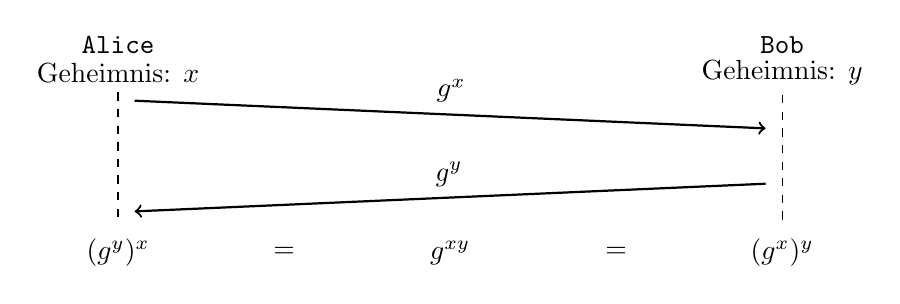
\begin{tikzpicture}[x=2em, y=2em]

			\draw (-6,0) node (Alice) {\texttt{Alice}};
			\draw (-6,-0.5) node (AliceSk) {Geheimnis: $x$};
			\draw (6,0) node (Bob) {\texttt{Bob}};
			\draw (6,-0.5) node (BobSk) {Geheimnis: $y$};
			
			% Lebenslinien
			\draw[dashed] (AliceSk) -- (-6,-3.25);
			\draw[dashed] (BobSk) -- (6,-3.25);
			
			% Pfeile fuer Nachrichten
			\textbf{\draw[->, thick] (-5.7,-1) -- (5.7,-1.5) node[sloped,above,pos=0.5] {$g^x$};}
			\textbf{\draw[->, thick] (5.7,-2.5) -- (-5.7,-3) node[sloped,above,pos=0.5] {$g^y$};}	
			
			% Beschriftung Ergebnis
			\draw (-6, -3.75) node {$(g^y)^x$};
			\draw (-3, -3.75) node {$=$};
			\draw (0, -3.75) node  {$g^{xy}$};
			\draw (3, -3.75) node  {$=$};
			\draw (6, -3.75) node  {$(g^x)^y$};

		\end{tikzpicture}
	\end{center}
	\caption{Diffie-Hellman-Schlüsselaustausch}
	\label{fig:keyex:dh}
\end{figure}
\FloatBarrier


\subsection{Transport Layer Security (TLS)}
Ziel ist, ein sicheres Verschlüsselungsverfahren für die Kommunikation über ein unsicheres Netzwerk zu ermöglichen.

\subsubsection{TLS-Handshake}

\begin{figure}[h]
\begin{center}
\unitlength=1mm
\linethickness{0.4pt}
\hspace{-3 cm}
	\begin{picture}(120,150)(-10,0)
		\put(20,143){\makebox(0,0)[cb]{\texttt{Client}$_{sk_C, pk_C}$}}
		\put(100,143){\makebox(0,0)[cb]{\texttt{Server}$_{sk_S, pk_S}$}}
	
		\put(20,2){\line(0,1){140}}
		\put(100,2){\line(0,1){140}}
		
		\put(5,131){\makebox(0,0)[cb]{berechne}}
		\put(5,127){\makebox(0,0)[cb]{Zufallszahl $R_C$}}
		\put(60,123){\makebox(0,0)[cb]{\emph{client\_hello}(Liste$_{Algorithmen}$, $R_C$)}}
		\put(20,122){\vector(1,0){80}}
	
		\put(117,118){\makebox(0,0)[cb]{berechne}}
		\put(117,114){\makebox(0,0)[cb]{Zufallszahl $R_S$}}
		\put(60,110){\makebox(0,0)[cb]{\emph{server\_hello}(Auswahl$_{Algorithmen}$, $R_S$)}}
		\put(100,109){\vector(-1,0){80}}
		
		\put(60,100){\makebox(0,0)[cb]{Server-Zertifikat (inkl. $pk_S$)}}
		\put(100,99){\vector(-1,0){80}}
		\put(60,94){\makebox(0,0)[cb]{Anfrage Client-Zertifikat}}
		\put(100,93){\vector(-1,0){80}}
		
		\put(3,87){\makebox(0,0)[cb]{überprüfe}}
		\put(3,84){\makebox(0,0)[cb]{Server-Zertifikat}}
		
		\put(60,80){\makebox(0,0)[cb]{Client-Zertifikat (inkl. $pk_C$)}}
		\put(20,79){\vector(1,0){80}}
	
		\put(3,73){\makebox(0,0)[cb]{berechne Hash $H$}}
		\put(3,69){\makebox(0,0)[cb]{aller bisherigen}}
		\put(3,66){\makebox(0,0)[cb]{Nachrichten}}
		\put(60,62){\makebox(0,0)[cb]{$SIG(sk_C, H)$}}
		\put(20,61){\vector(1,0){80}}
		
		\put(117,55){\makebox(0,0)[cb]{überprüfe $H$}}
		\put(117,51){\makebox(0,0)[cb]{und Signatur}}
		
		\put(3,55){\makebox(0,0)[cb]{berechne}}
		\put(3,51){\makebox(0,0)[cb]{Zufallszahl \emph{PMS}}}
		\put(60,47){\makebox(0,0)[cb]{$ENC(pk_S, \textit{PMS})$}}
		\put(20,46){\vector(1,0){80}}
		
		\put(3,40){\makebox(0,0)[cb]{berechne \emph{MS}}}
		\put(3,36){\makebox(0,0)[cb]{aus $R_C$, $R_S$, \emph{PMS}}}
		
		\put(117,40){\makebox(0,0)[cb]{berechne \emph{MS}}}
		\put(117,36){\makebox(0,0)[cb]{aus $R_C$, $R_S$, \emph{PMS}}}
		
		\put(60,32){\makebox(0,0)[cb]{\emph{ChangeCipherSpec}}}
		\put(20,31){\vector(1,0){80}}
		
		\put(60,26){\makebox(0,0)[cb]{\emph{Finished}}}
		\put(20,25){\vector(1,0){80}}
	
		\put(60,16){\makebox(0,0)[cb]{\emph{ChangeCipherSpec}}}
		\put(100,15){\vector(-1,0){80}}
		
		\put(60,10){\makebox(0,0)[cb]{\emph{Finished}}}
		\put(100,9){\vector(-1,0){80}}
	
	\end{picture}
\end{center}
\caption{Vereinfachter Ablauf eines SSL/TLS-Handshakes mit beidseitiger
	Authentifikation.} 
\label{fig:keyex:tls-handshake}
\end{figure}
\FloatBarrier

\subsubsection{Angriffe auf TLS}
Unter Verwendung einer idealen Verschlüsselung ist TLS sicher. Allerdings mussten konkrete Implementierungen als Reaktion auf veröffentlichte Angriffe immer wieder gepatcht werden.

\begin{itemize}
	\item \texttt{ChangeCipherSpec}-Drop: Angreifer unterdrückt den Aufruf des Clients, ab jetzt verschlüsselt zu kommunizieren. Falls der Server sofort danach Nutzdaten schickt, werden diese nicht verschlüsselt.
	\item Angriffe auf das Padding
	\item \texttt{CRIME}: Bei eingeschalteter Kompression kann ein aktiver Angreifer mit vielen Wiederholungen gezielt Klartexte rekonstruieren
	\item Logjam: Downgrade-Angriff
\end{itemize}



\section{Identifikationsprotokolle}



\section{Zero-Knowledge}
Voraussetzungen:
\begin{itemize}
	\item Verifier V lernt \(sk_P\) nicht (der geheime Schlüssel von \(P\))
	\item Prover P beweist, dass er \(sk_P\) kennt
\end{itemize}


\subsection{Zero-Knowledge-Eigenschaften}
\begin{itemize}
	\item V soll nichts über \(sk_P\) lernen, auch wenn er \(pk_P\) bereits kennt (\(pk_P\) ist mit \(sk_P\)) verknüpft
	\item Beispiel ElGamal: \(sk_P = x\) und \(pk_P = g^x\)
	\item Verwendung eines Simulators \(\mathcal{S}\), der die selbe Ausgabe erzeugt wie \(P\), jedoch ohne mit \(P\) kommuniziert zu haben
\end{itemize}

\paragraph{Ununterscheidbarkeit} Zwei Verteilungen \(X\) und \(Y\) sind ununterscheidbar, wenn für alle PPT-Algorithemn die Differenz \(Pr\big\lbrack\mathcal{A}(^k,x) ) 1 : x\leftarrow X\big\rbrack - Pr\big\lbrack\mathcal{A}(1^k,y) = 1 : y\leftarrow Y\big\rbrack\) vernachlässigbar in \(k\) ist. Intuitiv sind also Elemente aus \(X\) nicht effizient von Elementen aus \(Y\) unterscheidbar

\paragraph{Zero-Knowledge} Ein PK-Identifikationsprotokoll \(\big(GEN,P,V\big)\) ist Zero-Knowledge (ZK), falls für jeden PPT-Algorithmus \(\mathcal{A}\) (der Angreifer) ein PPT-Algorithmus \(\mathcal{S}\) (der Simulator) existiert, so dass die folgenden Verteilungen uunterscheidbar sind (wobei \((pk,sk) \leftarrow GEN(1^k)\)):
\[\langle P(sk),\mathcal{A}(1^k,pk)\rangle~~~~~~und~~~~~~(Ausgabe~von)~\mathcal{S}(1^k,pk)\]


\subsection{Commitments}
\begin{itemize}
	\item Hiding-Eigenschaft: \(COM\big(M;R\big)\) verrät zunächst keinerlei Informationen über \(M\)
	\item Binding-Eigenschaft: \(COM\big(M;R\big)\) legt den Ersteller des Commitments auf \(M\) fest, d.h. der Ersteller kann später nicht glaubhaft behaupten, dass \(M' \neq M\) zur Erstellung des Commitments verwendet wurde
\end{itemize}



\section{Benutzerauthentifikation}

\subsection{Kompression von Hashtabellen}
Anstelle einer vollständigen Liste aller möglichen Passwörter speichert
man nun eine Menge von $n$ Hashketten. Diese kann man tabellarisch darstellen:

\begin{figure}[h]
	\begin{gather*}
		(H(pw_{1,1}),pw_{1,1}) \xrightarrow{f}
		(H(pw_{1,2}),pw_{1,2}) \xrightarrow{f}\ldots\xrightarrow{f} (H(pw_{1,m}),pw_{1,m})\\
		(H(pw_{2,1}),pw_{2,1}) \xrightarrow{f} (H(pw_{2,2}),pw_{2,2}) \xrightarrow{f}\ldots\xrightarrow{f}
		(H(pw_{2,m}),pw_{2,m})\\ 
		\vdots\\ 
		(H(pw_{n,1}),pw_{n,1}) \xrightarrow{f}
		(H(pw_{n,2}),pw_{n,2}) \xrightarrow{f}\ldots\xrightarrow{f} (H(pw_{n,m}),pw_{n,m})
	\end{gather*}
	\caption{Tabellarische Darstellung von $n$ Hashketten der Länge
		$m$.}
\end{figure}

Gespeichert werden von diesen Hashketten nur die Startpassworte sowie die letzten Hashwerte. Die Tabelle wird nach Hashwerten sortiert. In komprimierter Form ergibt dies:

\begin{table}[!h]
	\begin{equation*}
		\begin{array}{|c|c|} \hline pw_{1,1} & H(pw_{1,m})\\
			\hline pw_{2,1} & H(pw_{2,m})\\
			\hline
			\vdots & \vdots \\
			\hline
			pw_{n,1} & H(pw_{n,m})\\
			\hline
		\end{array}
	\end{equation*}
	\caption{Die komprimierte Hashtabelle.}
\end{table}

Problem: Es kann passieren, das mehrere Hashketten, die mit verschiedenen Passworten starten, "`zusammenlaufen"'.

\subsubsection{Vorgehen}
\begin{itemize}
	\item Gegeben: Ein Hashwert
	\item Prüfe, ob der Hashwert in der komprimierten Tabelle vorkommt (also eines der letzten Hashkettenelemente ist)
	\item Falls ja: Berechne die komplette Hashkette, um den Ausgangswert des letzten Hashvorgangs zu erhalten
	\item Falls nein: % TODO
\end{itemize}



\section{Zugriffskontrolle}

\subsection{Das Bell-LaPadula-Modell}
\begin{itemize}
	\item Dynamisches Modell zur Zugriffskontrolle
	\item Bestandteile: Menge von Subjekten \(\mathcal{S}\), Menge von Objekten \(\mathcal{O}\), Menge \(\mathcal{A} = \{\texttt{read},\texttt{write},\texttt{append},\texttt{execute}\}\) von Zugriffsoperation, halbgeordnete Menge \(\mathcal{L}\) von Sicherheitsleveln
	\item Ein Systemzustand ist sicher, wenn die folgenden Eigenschaften erfüllt sind
	\item Sieht kein dynamisches Anpassen der Zugriffskontrollmatrix vor
\end{itemize}

\paragraph{Discretionary-Eigenschaft (ds-Eigenschaft)}
Alle Anfragen müssen konsistent mit der Zugriffsmatrix sein. Ein Systemzustand \((B,M,F)\) hat die ds-Eigenschaft, falls
\[\forall\big(s,o,a\big) \in B : a \in m_{s,o}.\]

\paragraph{Simple-Security-Eigenschaft (ss-Eigenschaft)}
Kein Subjekt darf lesend auf Objekte zugreifen, deren Sicherheitslevel das maximale Sicherheitslevel des zugreifenden Subjekts übersteigt. Ein Systemzustand \((B,M,F)\) hat die ss-Eigenschaft, falls
\[\forall\big(s,o,\texttt{read}\big) \in B : f_s(s) \geq f_o(o).\]

\paragraph{Star-Eigenschaft (\(\star\)-Eigenschaft)}
Subjekte dürfen lediglich in Objekte schreiben deren Sicherheitslevel mindestens genauso hoch sind (verhindert Informationsweitergabe "`nach unten"'). Ein Systemzustand \((B,M,F)\) hat die \(\star\)-Eigenschaft, falls
\[\forall\big(s,o,\{\texttt{write},\texttt{append}\}\big) \in B : f_o(o) \geq f_c(s).\]

Ist für eine gegebene \texttt{read}-Anfrage die ds-Eigenschaft und die ss-Eigenschaft erfüllt, wird das aktuelle Sicherheitslevel angepasst:
\[f_c(s) = max\big\{f_c(s),f_o(o)\big\}\]

\subsubsection{Nachteile}
\begin{itemize}
	\item Die aktuellen Sicherheitslevel werden nie herabgesetzt (Subjekte können in der Regel nicht gezwungen werden, gelesene Informationen zu vergessen)
	\item Subjekte können auf Objekte mit höherem Sicherheitslevel schreibend zugreifen
\end{itemize}


\subsection{Das Chinese-Wall-Modell}
\begin{itemize}
	\item Dynamisches Modell zur Zugriffskontrolle
	\item Ziel: Verhindern von Interessenskonflikten beim Zugriff auf Daten verschiedener Firmen, beispielsweise bei einer Beratungsunternehmen mit verschiedenen, teilweise in Konflikt stehenden Kunden
	\item \textbf{Bestandteile}
	\begin{itemize}
		\item Menge von Firmen \(\mathcal{C}\), Menge von Beratern \(\mathcal{S}\), Menge von Objekten \(\mathcal{O}\)
		\item Menge \(\mathcal{A} = \{\texttt{read},\texttt{write}\}\) von Zugriffsoperation
		\item Funktion \(y: \mathcal{O} \rightarrow \mathcal{C}\), die jedem Objekt seine Firma eindeutig zuweist
		\item Funktion \(x: \mathcal{O} \rightarrow \mathcal{P}(\mathcal{C})\), die jedem Objekt die Menge an Firmen zuweist, mit denen es in Konflikt steht
	\end{itemize}
\end{itemize}

\paragraph{Simple-Security-Eigenschaft (ss-Eigenschaft)}
Ein Konflikt entsteht, falls \(s\) in der Vergangenheit bereits Zugriff auf ein Objekt hate, das in Konflikt mit \(y(o)\) steht. Die Eigenschaft gilt, falls \(\forall o' \in \mathcal{O}\), auf die \(s\) schon Zugriff hatte, gilt:
\[y(o) = y(o') \vee y(o) \notin x(o').\]

\paragraph{Star-Eigenschaft}
Eine Schreibanfrage eines Beraters soll nur dann erlaubt werden, falls alle von ihm zuvor gelesenen Objekte entweder aus der gleichen Firma stammen oder mit keiner Firma in Konflikt stehen. Eine Anfrage hat die Eigenschaft, falls \(\forall o' \in \mathcal{O}\), auf die \(s\) schon lesend zugegriffen hat, gilt:
\[y(o) = y(o') \vee x(o') = \emptyset.\]



\section{Analyse umfangreicher Protokolle}



\section{Implementierungsprobleme}

\subsection{Bufferoverflow}
\begin{itemize}
	\item In C/C++ (und weiteren Programmiersprachen) finden Pufferzugriffe ohne Größenüberprüfungen statt
	\item Auch bei Zugriffen außerhalb des Speicherbereichs kommt es zu keinem Programmfehler
	\item Angreifer können gezielt Speicherbereiche überschreiben
	\item Befindet sich der übergelaufene Puffer auf dem Stack, kann sogar die Rücksprungadresse überschrieben werden \(\rightarrow\) wird diese überschrieben, so kann der Programmfluss gelenkt werden
	\item \textbf{Gegenmaßnahmen}
	\begin{itemize}
		\item Explizites Prüfen der Puffergröße. Kann auch automatisch von bestimmten Funktionen (beispielsweise \texttt{strncat} oder \texttt{strncopy}) oder Programmiersprachen (beispielsweise Java) durchgeführt werden. Allerdings sehr aufwendig bei großen Programmen nachzurüsten
		\item \textit{Stack Canaries}: Zufällige Dummywerte, die vor der Rücksprungadresse platziert werden. Der Compiler fügt vor jedem Rücksprung noch einige Befehle ein, die Prüfen, ob der Stack Canary verändert worden ist
		\item \textit{Data Execution Prevention}: Prozessor erzwingt Trennung von Code- und Speicherbereichen. Dadurch kann der vom Angreifer eingeschleuste Code nicht ausgeführt werden
		\item \textit{Address Space Layout Randomization}: Das Betriebssystem platziert Speicherbereiche zufällig. Dadurch kann der Angreifer entsprechende Bereiche nicht erkennen (wo beispielsweise die Rücksprungadresse liegt)
	\end{itemize}
\end{itemize}


\subsection{SQL-Injection}
\begin{itemize}
	\item Ziel des Angreifers: "`Platzieren"' von bösartigen SQL-Befehlen über Eingabemasken
	\item Beispiel: Aus \texttt{SELECT * FROM cd WHERE album='\$album';} wird \texttt{SELECT * FROM cd WHERE album=''; DROP TABLE cd;}. Die Datenbank interpretiert die Abfrage als zwei Anweisungen und führt beide hintereinander aus
	\item Gegenmaßnahmen: Gründliche Überprüfung der Benutzereingaben; Escapen von Sonderzeichen (beispielsweise über \texttt{mysql\_escape\_string}); Verwenden von \textit{Prepared Statements}
\end{itemize}


\subsection{Cross Site Scripting}
\begin{itemize}
	\item Injízieren von HTML-Elementen in eine Webseite. Über JavaScript kann diese dann vollständig kontrolliert werden. So können beispielsweise Login-Daten abgegriffen werden
	\item Gegenmaßnahme: Maskieren aller Benutzereingaben (\texttt{htmspecialchars}), damit sie nicht vom Browser als HTML interpretiert werden können
\end{itemize}


\subsection{Denial of Service}
\begin{itemize}
	\item Ziel: Lahmlegen bestimmter Dienste durch eine sehr große Menge parallele Anfragen
	\item \textit{SYN-Flooding}: Initiierung des (clientseitigen) TCP-Handshaken mit \texttt{SYN}-Paket, ohne abschießend \texttt{ACK} zu senden. So wartet der Server nach Empfang von \texttt{SYN} auf \texttt{ACK} und reserviert Ressourcen
\end{itemize}


\begin{landscape}
\setlength\extrarowheight{5pt}

\section{Appendix A: Sicherheitsbegriffe}
\begin{table}[H]
\begin{tabularx}{\linewidth}{|l|X|X|X|}
\hline
& \textbf{Semantische Sicherheit} & \textbf{IND-CPA-Sicherheitsbegriff} & \textbf{IND-CCA-Sicherheitsbegriff} 	\\
\hline
\textbf{Begriff} &
Alle Informationen, die mit \(C\) effizient über \(M\) berechnet werden können, sind auch ohne das Chiffrat berechenbar. &
\textit{Indistinguishability under chosen-plaintext attacks}: Ein polynomiell beschränkter Angreifer \(\mathcal{A}\) kann die Chiffrate nicht von selbst gewählten Klartexten unterscheiden. &
\textit{Indistinguishability under chosen-ciphertext attacks}\\
\hline
\textbf{Definition} &
Ein Verfahren ist genau dann semantisch sicher, wenn es IND-CPA-sicher ist.&
\(\mathcal{A}\) kann sich zu jedem Zeitpunkt jedes beliebige \(M\) vom Orakel verschlüsseln lassen.
\begin{enumerate}
	\item \(\mathcal{A}\) wählt verschiedene \(M_1\) und \(M_2\) gleicher Länge
	\item Challenger \(\mathcal{C}\) verschlüsselt zufällig einen der beiden Klartexte \(M_i\) mit \(i \in \{1,2\}\) und übergibt dieses \(C*\) an \(\mathcal{A}\)
	\item \(\mathcal{A}\) gewinnt, wenn er \(i\) korrekt rät
\end{enumerate}&
Verschlüsselungsorakel:
\begin{itemize}
	\item \(\mathcal{A}\) kann sich beliebige \(M\) verschlüsseln lassen
	\item \(\mathcal{A}\) darf sich, mit Ausnahme des in (2) erhaltenen \(C*\) jedes beliebige \(C\) verschlüsseln lassen
\end{itemize}
Verfahren:
\begin{enumerate}
	\item \(\mathcal{A}\) wählt verschiedene \(M_1\) und \(M_2\) gleicher Länge
	\item Challenger \(\mathcal{C}\) verschlüsselt zufällig einen der beiden Klartexte \(M_i\) mit \(i \in \{1,2\}\) und übergibt dieses \(C*\) an \(\mathcal{A}\)
	\item \(\mathcal{A}\) gewinnt, wenn er \(i\) korrekt rät
\end{enumerate}\\
\hline
\textbf{RSA/ElGamal}&
Da beide Verfahren nicht IND-CPA-sicher sind, sind sie auch nicht semantisch sicher.&
Beide Verfahren sind deterministisch und können daher nicht IND-CPA-sicher sein.&
RSA-OAEP ist IND-CCA-sicher.\\
\hline
\end{tabularx}
\end{table}


\begin{table}[H]
\begin{tabularx}{\linewidth}{|l|X|X|}
\hline
& \textbf{Symmetrische EUF-CMA-Sicherheit} & \textbf{Asymmetrische EUF-CMA-Sicherheit} \\
\hline
\textbf{Begriff} &
\textit{Existential Unforgeability}: Es darf keine Nachricht geben, für die \(\mathcal{A}\) eine Fälschung erstellen kann &
\\
\hline
\textbf{Beschreibung} &
\begin{enumerate}
	\item \(\mathcal{A}\) erhält Zugriff an ein Signaturorakel \(SIG(K,\cdot)\), an das er polynomiell viele Nachrichten zum Signieren schicken darf
	\item \(\mathcal{A}\) gibt ein Nachrichten-Signatur-Paar als (potentielle) Fälschung aus
	\item \(\mathcal{A}\) gewinnt, wenn die Signatur korrekt ist und er sich diese Nachricht nicht vom Orakel hat signieren lassen
\end{enumerate} &
\begin{enumerate}
	\item \(\mathcal{C}\) generiert ein Schlüsselpaar \((pk,sk) \leftarrow GEN(1^k)\) für sich
	\item \(\mathcal{A}\) erhält Zugriff auf ein Signturorakel \(SIG(pk,\cdot)\), an das er polynomiell viele Nachrichten schicken darf
	\item \(\mathcal{A}\) gibt ein Nachrichten-Signatur-Paar als (potentielle) Fälschung aus
	\item \(\mathcal{A}\) gewinnt, wenn die Signatur korrekt ist und er sich diese Nachricht nicht vom Orakel hat signieren lassen
\end{enumerate}
\\
\hline
\end{tabularx}
\end{table}

\end{landscape}
